
\subsection{Klassediagram}


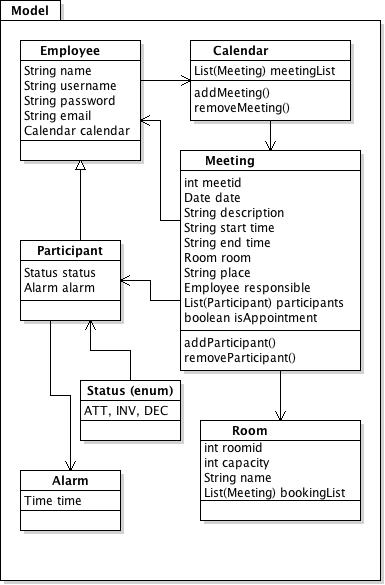
\includegraphics[width=\textwidth]{klassediagram.jpg}

Dette er sånn vi ser for oss modellene til applikasjonen, og hvordan dataobjektene interagerer med hverandre. Så hvis en bruker skal opprette et nytt møte, har vi et panel i GUI med inputfelter, og møtemodellen må oppdateres i backend i henhold til inputen brukeren sender inn. Her må vi ha opprettet en kobling til serveren som kjører med databasen slik at databasen oppdateres når en endring skjer. 

Alle avtaler og møter er to sider av samme sak, så vi har bare en Meeting-klasse med en variabel som sier om det er en avtale eller et møte. Det er et møte dersom det er to eller flere deltakere. 

Participant arver fra Employee slik at vi kan ha en status-variabel som forteller om møtedeltakeren deltar, deltar ikke eller ikke har svart. 

